\documentclass[11pt,a4paper]{article}
\usepackage[utf8]{inputenc}
\usepackage[T1]{fontenc}
\usepackage{lmodern}
\usepackage[french]{babel}
\usepackage[margin=1in]{geometry} 
\usepackage[parfill]{parskip}
\usepackage{amsfonts}
\usepackage{amssymb}
\usepackage{amsmath}
% add system ( emphased equation )
\usepackage{empheq}
%mfrac
\usepackage{csquotes}
\usepackage{nccmath}
\usepackage{xcolor}
\usepackage{float}
\usepackage{graphicx}
\usepackage{hyperref}
\usepackage{caption}
\usepackage{subcaption}
%\usepackage{csquotes}
\usepackage{enumitem}
\usepackage{multirow}
\usepackage{longtable}
%\usepackage[style=ieee]{biblatex}
\usepackage{todonotes}
\usepackage{pdfpages}
\setlist[itemize,1]{label=$\circ$}
\setlist[enumerate,1]{label=(\alph*), ref=\thesection(\alph*)}
\setlist[enumerate,2]{label=\roman*., ref=\thesection(\alph{enumi}).\roman*}
\newcommand{\magikpdf}[2]{
        \includepdf[pages=-,width=0.9\paperwidth,pages={1},clip,
pagecommand={#1}]{#2} % wierd wizard stuff
}
\usepackage{lipsum}
\usepackage{listings}
\newcommand{\dd}{d_1}
\newcommand{\dt}{d_T}
\newcommand{\da}{d_A}
\newcommand{\blank}{\mathrel{\underline{\hspace{2em}}}}
\newcommand{\Ma}{M_A}
\newcommand{\Mt}{M_T}
\newcommand{\Na}{N_A}
\newcommand{\Nt}{N_T}
\newcommand{\ddd}{d_2}
\newcommand{\Fr}{F_r}
\newcommand{\Ft}{F_t}
\newcommand{\Fa}{F_a}
\DeclareMathOperator{\Var}{Var}
\newcommand{\cotan}{\mathrm{cotan}}
\begin{document}
\begin{titlepage}
	\begin{minipage}{0.5\textwidth}
		\begin{flushleft}
			
\includegraphics[height=2.3cm]{template/Im1.PNG}
		\end{flushleft}
	\end{minipage}
	\begin{minipage}{0.5\textwidth}
		\begin{flushright}
			
\includegraphics[height=1.9cm]{template/Im2.PNG}
		\end{flushright}
	\end{minipage} \\ [3cm]
	\begin{center}
		\textsc{\LARGE Université de Liège}\\[0.5cm]
		\textsc{\Large Faculté des Sciences Appliquées}\\[3.0 cm]
		\noindent\rule{\textwidth}{0.4mm} \\[.7cm]
		\textsc{\LARGE SYST0002 }\\[0.7cm]
		\textsc{\LARGE  Introduction aux signaux et systèmes}\\[0.7cm]
		\textsc{\LARGE  Projet}\\[0.7cm]
		%\textsc{\LARGE\textit{ }}\\[0.5cm]
	\end{center}
	\noindent\rule{\textwidth}{0.4mm}
	\vspace*{10mm}
	\textsc{\large DELBARRE} \large Loïc (S215072) \\[1mm]
	\textsc{\large JACQUEMIN} \large Justin (S224395) \\
	\begin{center}
		\vfill
		{\large Bachelier Ingénieur Civil
			\\[.3cm]
			Année Académique 2024-2025}
	\end{center}
\end{titlepage}
\setcounter{tocdepth}{3}
\pagebreak
%\listoffigures
%\newpage
\tableofcontents
\newpage

%%%%%%%%%%%%%%%%%%%%%%%%%%%%%%%%%%%%%%%%%%%%%%%%%%%%%%%%%%%%%%%%%%%%%%%

\section{Part 1: modèle d'état, linéarisation et simulations}
%donnez toutes les nonlinéarités et les fonctions non-linéaires sont appliquées sur quoi ? Le temps ?, un signal ? Lequel ?
\subsection{linéarité du modèle dynamique}
Le système n’est pas linéaire, car il ne respecte pas les principes de superposition et d’homogénéité, en raison de la présence de fonctions non linéaires ( sin , tan , arctan) dans sa dynamique ainsi que de l'adition de variable d'état $\theta(t)$ à une fonction d'entrée $\delta(t)$ dans un sinus .

Par conséquent, le système ne satisfait pas les propriétés de superposition et d’homogénéité qui caractérisent les systèmes linéaires.
\subsection{paramètre du système}
Pour tout les signaux mentionnés , nous supposeront que $t \in \mathbb{R}^+$ vu qu'il s'agit du temps.
\begin{itemize}
	\item entrées : $\delta(t)$
	      Le delta est associé à l'orientation des roue par rapport à l'axe du véhicule en fonction du temps.Son image appartient à l'intervale $[-\dfrac{\pi}{2},\dfrac{\pi}{2}]$
	\item variables d'états : $y(t),\theta(t)$
    \begin{itemize}
      \item $y(t)$ représente l'évolution temporelle de la position selon l'axe vertical.Il n'y a pas de contrainte dans l'énoncé, on peut donc supposer que son domaine de définition ainsi que son image appartiennent à $\mathbb{R}$
      \item $\theta(t)$ représente l'évolution temporelle de l'orientation du véhicule dans l'espace.Vu qu'il s'agit d'un angle , on peut raisonablement restreindre son image à l'intervale $ [ 0 , 2\pi]$
    \end{itemize}
	      $\theta$ quant'à lui représente l'évolution temporelle de l'orientation du véhicule dans l'espace.Vu qu'il s'agit d'un angle , on peut raisonablement restreindre son image à l'intervale $[ 0,2\pi]$
	\item constantes: a , b , $v_0$ \begin{itemize}
	 \item 
    a est la distance entre l'axe arrière et le centre de masse du véhicule. 
    \item b , la distance entre l'axe des roues avant et celui des roues arrière.
    \item $v_0$ représente la vitesse du centre de masse.

	\end{itemize}
	\item sorties : $s(t)$
	      La sortie est la position selon l'axe vetical
\end{itemize}
\subsection{simulation du système}
\subsubsection{cas d'un mouvement avec les roues fixes}
\begin{figure}[!h]
	\centering
	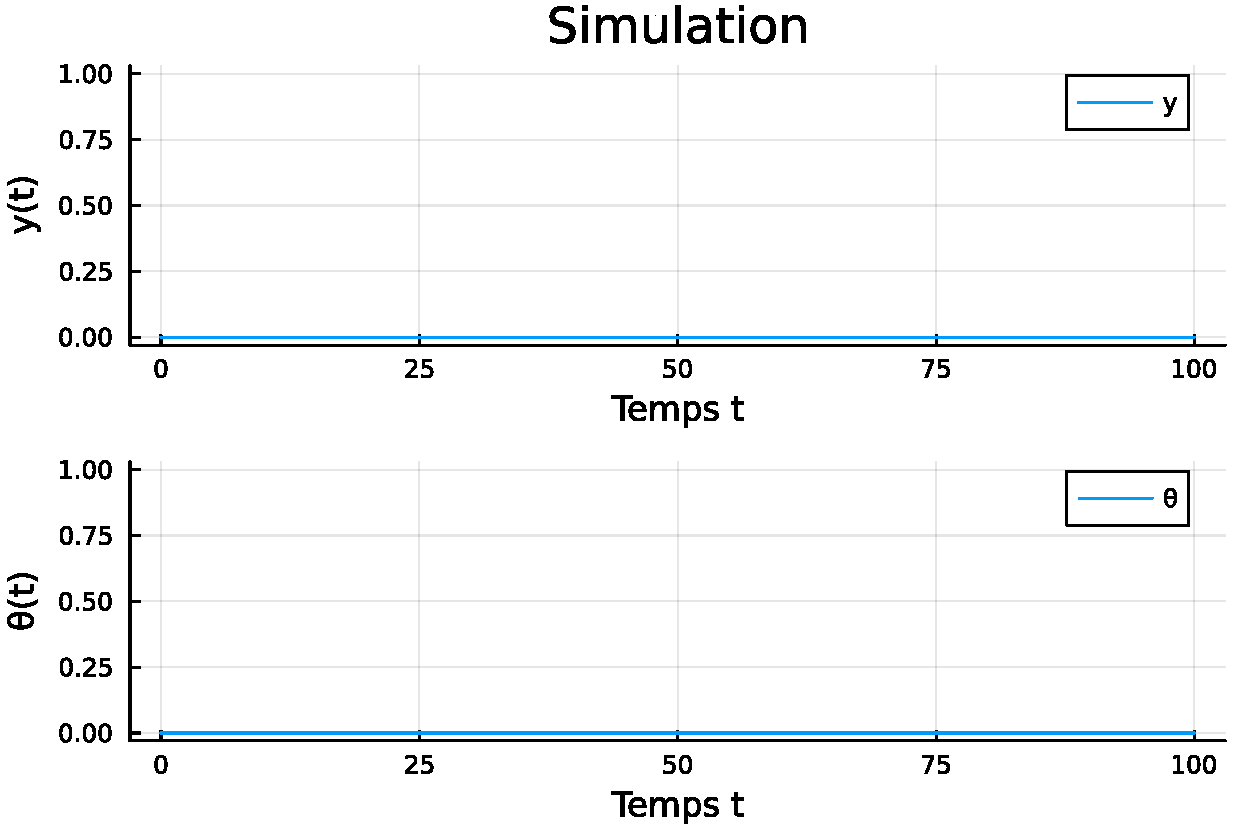
\includegraphics[width=0.5\linewidth]{../code/jlplots/Q1_3_zero.pdf}
\end{figure}
\newpage
\subsubsection{cas d'un mouvement dont les roues oscillent sinusoidalement}
\begin{figure}[!h]
	\centering
	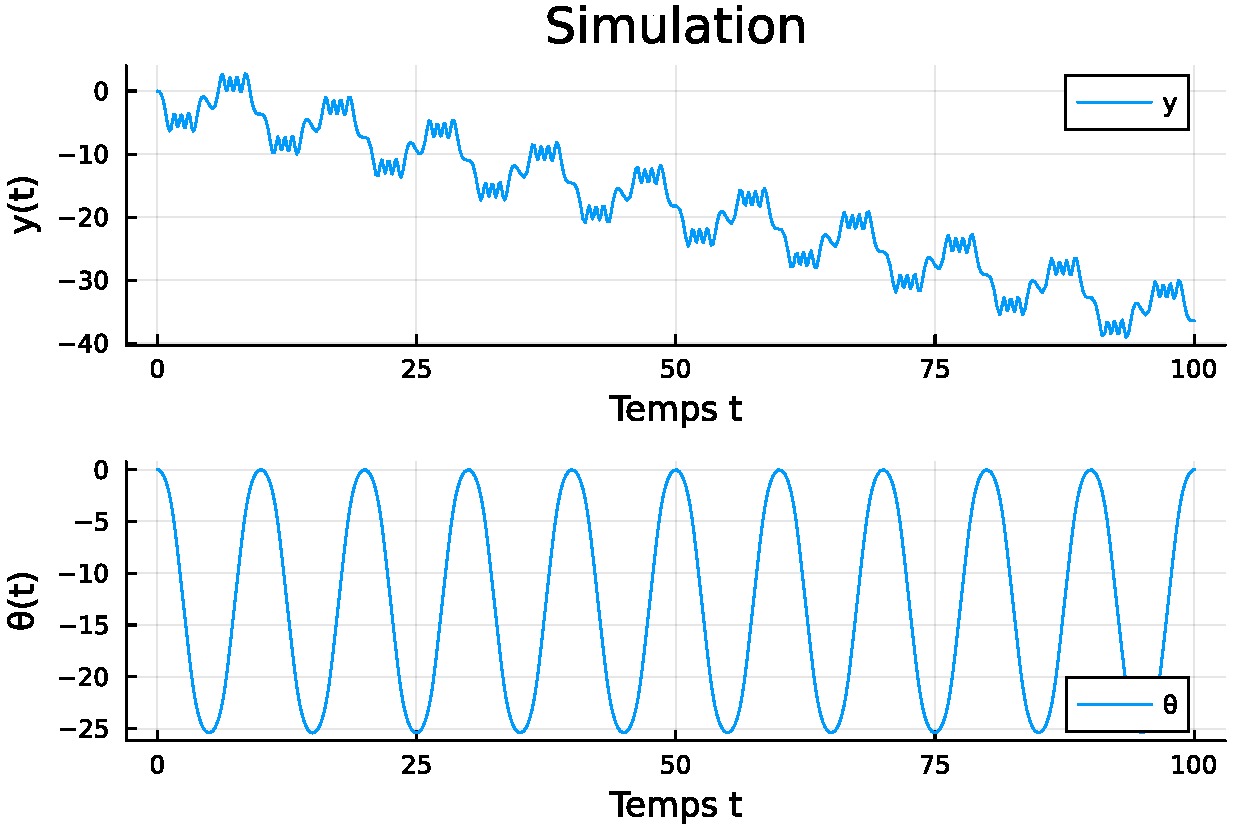
\includegraphics[width=0.5\linewidth]{../code/jlplots/Q1_3_delta.pdf}
\end{figure}
\subsection{Points d'équilibre du système}
\begin{displayquote}
Dans le cadre de ce rapport , nous utiliseront la notation $\dot y$ qui correspond à $\dfrac{d y}{dt}$.
\end{displayquote}
Afin de trouver les points d'équilibre du système de manière analytique il suffit de trouver :
\begin{equation}
	\begin{cases}
		\dot y=0 \\
		\dot \theta=0%= \dfrac{v_0 sin \alpha(\delta (t) )}{a}
	\end{cases}
\end{equation}
On trouve donc par la deuxième équation que
$$\delta(t) = k\pi \quad \text{avec} \quad k \in \mathbb{Z}$$
De là, en découle via la première équation que
$$\theta(t)=k\pi \quad \text{avec} \quad k \in \mathbb{Z}$$
On trouve donc dans le système deux point d'équilibre au vu des domaines et des images.On a donc $(\delta;\theta)=(0;0)$ ou bien $(\delta;\theta)=(0;\pi)$
\subsection{Matrice d'état A,B,C,D}
Afin de trouver les matrice d'état du système il faut se baser sur la méthode des dérivées.
On identifie aisément que :
\begin{equation}
	\begin{cases}
		f= v_0 \sin(\alpha(\delta(t)+\theta(t)) \\
		g= \dfrac{v_0 sin(\alpha(\delta(t))}{a}
	\end{cases}
\end{equation}
Les matrices sont donc calculé via les dérivées au point d'équilibre du système:
\begin{equation}
	\begin{cases}
		A= \begin{pmatrix}
			   0 & \pm v_0 \\
			   0 & 0
		   \end{pmatrix}       \\
		B= \begin{pmatrix}
			   \dfrac{\pm v_0 a}{b} \\
			   \dfrac{\pm v_0}{b}
		   \end{pmatrix} \\
		C= \begin{pmatrix}
			   1 & 0
		   \end{pmatrix}       \\
		D= \begin{pmatrix}
			   0
		   \end{pmatrix}
	\end{cases}
\end{equation}
Le système deviens dès lors :
$$
	\frac{d}{dt}
	\begin{pmatrix}
		y(t) \\
		\theta(t)
	\end{pmatrix}
	=
	\begin{bmatrix}
		0 & \pm v_0 \\
		0 & 0
	\end{bmatrix}
	\begin{pmatrix}
		y(t) \\
		\theta(t)
	\end{pmatrix}
	+
	\begin{bmatrix}
		\pm v_0 \frac{a}{b} \\
		\frac{\pm v_0}{b}
	\end{bmatrix}
	\delta(t).
$$
$$s(t)=\begin{bmatrix} 1 & 0 \end{bmatrix}
  \begin{bmatrix}y(t) \\ \theta(t) \end{bmatrix}
    + \begin{bmatrix}0 \end{bmatrix} \begin{bmatrix} \delta(t) \end{bmatrix}
$$

\subsection{nature des points d'équilibre}
Pour connaitre la nature des points d'équilibre , il suffit de calculer les valeurs propres de la matrice d'état A.
$$
\det(A - \lambda I) = 
\begin{vmatrix}
-\lambda &\pm v_0 \\
0 & -\lambda
\end{vmatrix}
= (-\lambda)(-\lambda) - (0)(v_0) = \lambda^2
$$
\todo[inline]{on ne peux rien dire sur la nature de tout les points d'équilibre ducoup ?}
Vu que ses valeurs sont nulles , on ne peux donc rien conclure concernant la stabilité du système \todo{marginalement stable ? }.

\subsection{simulation au point d'équilibre}



\begin{figure}[!h]
	\centering
	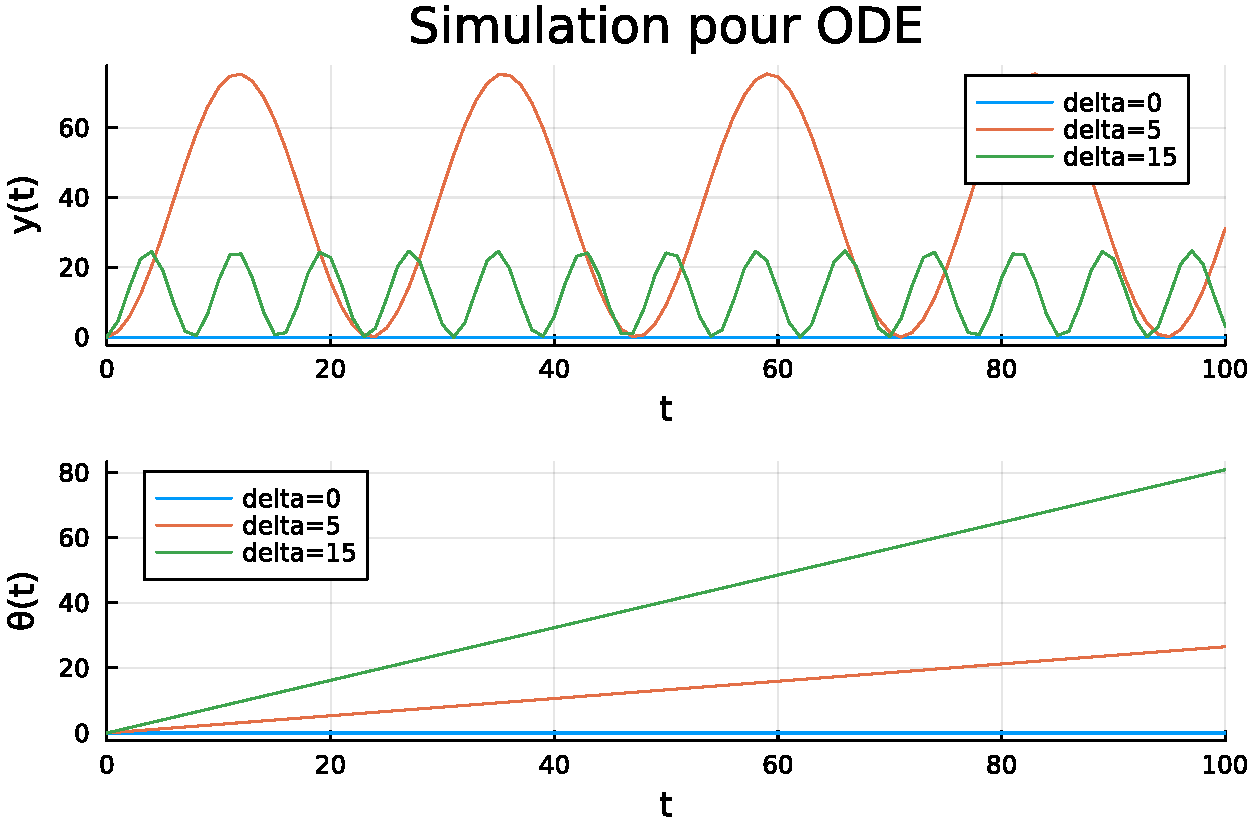
\includegraphics[width=0.5\linewidth]{../code/jlplots/Q1_7_ODE.pdf}
\end{figure}
\begin{figure}[!h]
	\centering
	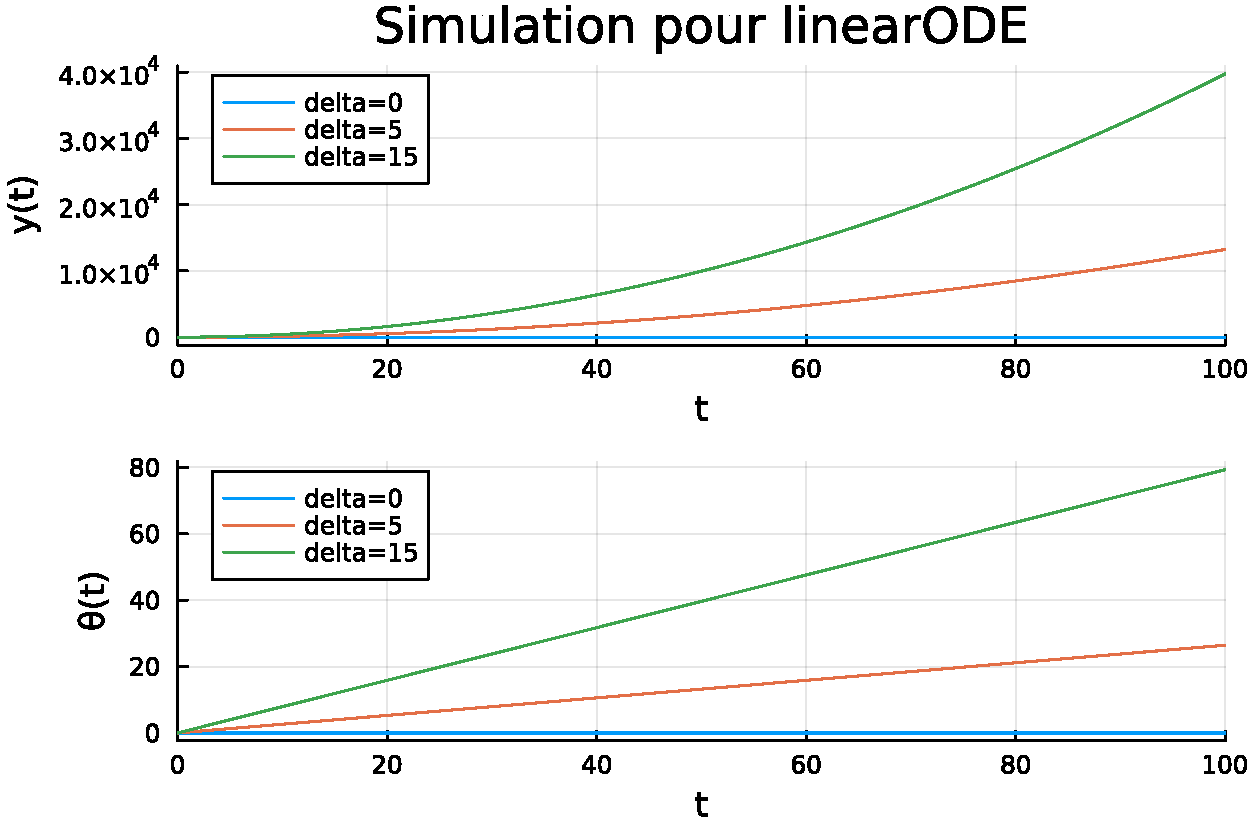
\includegraphics[width=0.5\linewidth]{../code/jlplots/Q1_7_linearODE.pdf}
\end{figure}
On peut constater que les fonctions non linéaire ont le même résultat que celle du modèle ABCD.
Vu que l'on fixe $\delta$ a une constante qui ne dépends pas du temps , 
Vu que $\delta$ étant constant, $\dot \theta$ l'est aussi et donc $\theta$ croit linéairement de pente . \\
Concernant $y(t)$ la situation est différente, on a une relation qui dépends de $\theta$ ainsi que d'une constante. On a donc un comportement "exponentiel".
la valeur de $\dot \theta$ n'est pas modifié au fur et a mesure du temps et donc pour $\theta>0 $ on appercois une augmentation de y(t) constante qui est représenté sur la courbe par la courbure exponentielle.

\subsection{trajectoire gaussienne}
\begin{figure}[!h]
  \begin{center}
    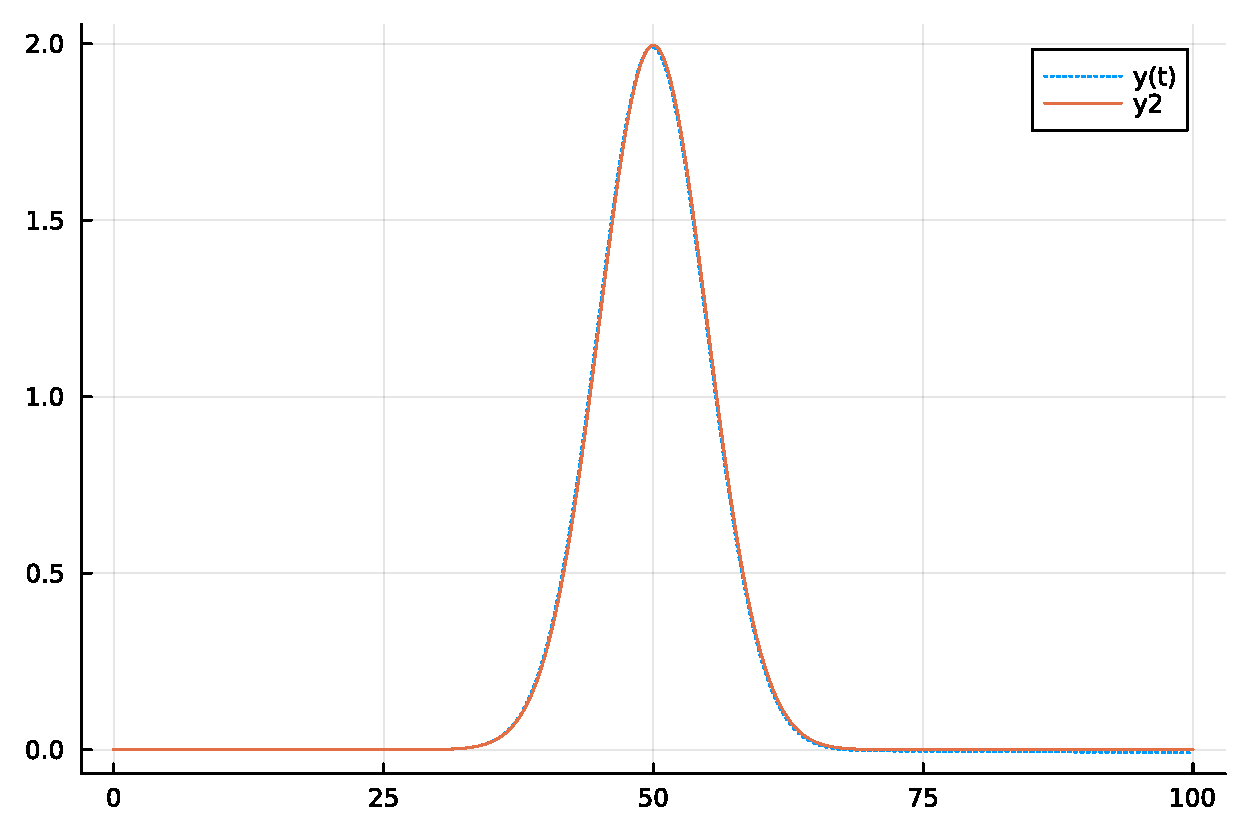
\includegraphics[width=0.95\textwidth]{../code/jlplots/Q1_8.pdf}
  \end{center}
  \caption{}\label{fig:Q1_8_gaussian}
\end{figure}

avec actuellement une MSE de 0.00010265487225667491
\todo[inline]{formuler ca correctement}
Afin de trouver la juste somme de gausiennes pour $\delta(t)$, différentes pistes s'offrent à nous.
\begin{itemize}
  \item 
La méthode analytique n'est pas envisageable au vu de la complexité du système et la méthode analytique sur le modèle linéarisé n'est pas suffisament proche de la réalité pour avoir du sens. 
\item 
\end{itemize}
Concernant la méthode numérique une approche naive serait de poser le problème comme étant une minimisation de la mean square error entre notre signal de sortie et notre signal d'entrée en fonction des parametres des gaussiennes. 
Le problème principal de cette approche est , que la fonction comporte beaucoup trop de minimum locaux sur sa topologie mais également que le nombre de parametre pouvant croitre , la minimisation serait d'autant plus couteuse. 
Pour palier à ce problème la première solution envisagée a été de bénéficier des symétrie du problèmes ainsi que des propriété des gaussiennes.
En effet on peut voir une gausienne comme étant un "coup de volant aller-retour",on constate donc qu'il y aurra besoin de 3 gaussiennes dont le parametre $\mu$ déterminerai le temps a la quelle celui ci serait effectué et $A$ la violence de celui ci. 
Pour réduire encore le nombre de paramêtre à 7, une des approche envisagée a été de supposer que deux coups de volant serait équidistant de 50 et l'un a 50. Concernant l'algorithme , les deux algoritme simple a implémenter sont la recherche aléatoire et la grid search. Au vu du nombre de dimension du problème une grid search aurrait pris beaucoup de temps avant de converger. C'est pour cela que nous sommes parti sur une recherche aléatoire. 



\subsubsection{résolution numérique}
On peut supposer le problème comme étant la minimization d'une fonction prennant en argument une matrice colone de taille 3n représentant les différents paramètre associé au différentes Gaussiennes et retournant le Mean square error comparé a la trajectoire attendue .
Actuellement nous avons fait tourner sans succès notre minimization pour des tailles de matrice allant jusqu'a 15 élément.
\subsubsection{recherche de paramètre}


Une première approche bête et naive serait de tester des combinaisons de n gausiennes  et de faire une minimisation sur 3n parametre.
Au vu du problème considéré une méthode de minimisation basée sur une dérivée ne fonctionnerai pas car la fonction présente beaucoup trop de minimum locaux.

Si l'on considère la fonction trajectoire que le véhicule doit avoir, on y remarque 3 " coup de volant". Un coup de volant peut se traduire par une fonction $\delta(t) $
similaire a une gausienne ou une parabole et dont le sens de la courbure indiquerai le sens du coup de volant.
Afin de simplifier encore le nombre de variable , on peut profiter des propriété des parametre d'une gaussienne, dans les 3 coups de volant , l'un semble centré en 50 et le deux autres semblent être équidistant à 50.Il en va de soit aussi dans l'intensité du coup de v 

\section{State-feedback controller, simulations et analyse de Fourier}
\subsection{}
\subsection{calcul des matrices d'état du système global}
En remplacant l'équation du controller dans celle du Plant , on obtient:
\begin{equation}
	\begin{cases}
		\dot x= (A-KB)x+BK_rr \\
		s= (C-KD)x+DK_rr
	\end{cases}
\end{equation}
Par identification,on remarque donc que : \\
\begin{equation}
	\begin{cases}
		\tilde{A} = A-BK= \begin{bmatrix} - k_1 V_0 \frac ab & v_0 - k_2v_0 \frac ab \\ -k_1 \frac {v_0} b & -k_2 \frac{v_0}b \end{bmatrix} \\
		\tilde{B} = K_rB= \begin{bmatrix} k_r v_0 \frac ab \\  k_r \frac{v_0}b \end{bmatrix}                                                \\
		\tilde{C} = C-DK= \begin{bmatrix} 1 & 0  \end{bmatrix}                                                                              \\
		\tilde{D} = K_rD = \begin{bmatrix}  0  \end{bmatrix}                                                                                \\
	\end{cases}
\end{equation}
\subsection{simulation du modèle \textit{control loop}}
% TODO rajouter graphs et donner conclusion 
\subsection{simulation avec une entrée sinusoidales}
\subsection{domaine fréquentiel}

Afin de se simplifier les notation , il suffit de définir un $\omega$ comme étant $2\pi f_{ref}$ avec $f_{ref}$ la fréquence de référence .  \\

\begin{align*}
	2sin(2\pi f t + \dfrac{\pi}{6}) &                                                                                                                                                                                              \\
	X(j\omega)=                     & 2 \int_{0}^{100} sin(\omega _{0}t + \phi)e^{j\omega t} dt                                                                                                                                    \\
	=                               & 2 \int_{\frac T2 - \frac T2} ^{\frac T2 + \frac T2} \dfrac{e^{j \omega _0 t}-e^{-j \omega _0 t}}{2j} e^{-j\omega t} dt                                                                       \\
	=                               & \frac 1j \int_{\frac T2 - \frac T2} ^{\frac T2 + \frac T2} e^{j (\omega _0 - \omega)t+j\phi }- e^{-j( \omega _0+ \omega)t-j\phi} dt                                                          \\
	=                               & \frac 1j \left [ \dfrac{e^{j(\omega_0-\omega)t+j\phi}}{j(\omega_0-\omega)}- \dfrac{e^{-j(\omega_0+\omega)t-j\phi}}{j(\omega_0+\omega)} \right] _{\frac T2 - \frac T2} ^{\frac T2 + \frac T2} \\
	=                               & \dfrac{e^{j\left((\omega _0-\omega)\frac T2 + \phi \right)}}{j^2(\omega _0 - \omega)} \left(e^{j(\omega _0- \omega)\frac T2 } -e^{-j(\omega _0- \omega)\frac T2 } \right)
	+ \dfrac{e^{-j\left((\omega_0+\omega)\frac T2+ \phi\right)}}{j^2(\omega _0 + \omega)}\left( e^{j(\omega_0 + \omega)\frac T2 } - e^{-j(\omega_0+\omega)\frac T2}\right)                                                         \\
	=                               & \dfrac{2e^{j\left((\omega _0-\omega)\frac T2 + \phi \right)}}{j(\omega _0 - \omega)} sin\left((\omega_0-\omega)\frac T2 \right)
	+ \dfrac{2e^{-j\left((\omega_0+\omega)\frac T2+ \phi\right)}}{j(\omega _0 + \omega)}sin\left((\omega_0+\omega)\frac T2\right)                                                                                                  \\
	=                               & -2je^{j\left((\omega _0-\omega)\frac T2 + \phi \right)}sinc\left((\omega_0-\omega)\frac T2 \right)
	- 2je^{-j\left((\omega_0+\omega)\frac T2+ \phi\right)}sinc\left((\omega_0+\omega)\frac T2\right)                                                                                                                               \\
\end{align*}
Au vu des sinus cardinaux , les peak se trouvent donc en $\omega =\pm\omega_0$.Autrement dit, $\omega=\pm 2 \pi f_{ref}$
\subsection{diagrammes d'amplitudes}
Au vu du signal de sortie que l'on obtient dans la partie 4 , il est assez visuel de voir qu'il s'agit d'une sinusoide d'amplitude et de fréquence visible.
Ici pour tracer numériquement on aurrait pu le faire a la main. Nous avons décidé de se baser sur la Discrete Fourier Transform ( DFT ) pour récupérer le graphique de fréquence.
\section{Fonction de transfert et diagrammes de Bode}
\subsection{fonction de transfert du système total}
Pour déterminer $H(s)$ , on peut se baser sur les matrices d'état
$\tilde{A},\tilde{B},\tilde{C},\tilde{D}$,ceci permettra de déterminer les pôles de H(s).Concernant sa stabilité , une fonction de transfert est dite stable si $\mathrm {Re} \{ p\}<0$on a donc : \\
$$H(s)=\tilde{C} \left (s \mathbb{I} _2 - \tilde{A} \right)^{-1} \tilde{B} + \tilde{D} $$
\begin{align*}
	H(s) & = \begin{bmatrix} 1 & 0  \end{bmatrix} \begin{bmatrix}  k_1 v_0  \frac ab +s & k_2v_0  \frac ab - v_0 \\ k_1 \frac {v_0} b & k_2 \frac{v_0}b+s \end{bmatrix}^{-1}
	\begin{bmatrix} k_r v_0 \frac ab \\  k_r \frac{v_0}b \end{bmatrix} + \begin{bmatrix}  0  \end{bmatrix}                                                                                                                         \\
	     & =\dfrac{1}{s^2 + \frac{v_0}b [a k_1 + k_2]s + \frac{k_1 v_0 ^2}b} \begin{bmatrix} 1 & 0 \end{bmatrix} \begin{bmatrix}k_2 \frac{v_0}b+s & v_0 -k_2 v_0 \frac ab \\ - k_1 \frac{v_0}b & k_1 v_0 \frac ab +s \end{bmatrix}
	\begin{bmatrix} k_r v_0 \frac ab \\ k_r \frac {v_0}b \end{bmatrix}                                                                                                                                                             \\
	     & =\dfrac{k_r v_0}{b}\dfrac{as+v_0}{s^2 + \frac{v_0}b [a k_1 + k_2 ]s + \frac{k_1 v_0 ^2}b}                                                                                                                                \\
	\text{en remplacant par les valeurs on obtient;}                                                                                                                                                                               \\
	     & = \dfrac{0.440s + 4}{s^2 + 2 s + 4}
\end{align*}
Au vu de l'alure de $H(s)$ il est aisé de remarqué son zéros en $\frac{-b}{a k_r}$
Cette fonction de control est également trouvé directement dans le code.

\begin{figure}[!h]
  \begin{center}
    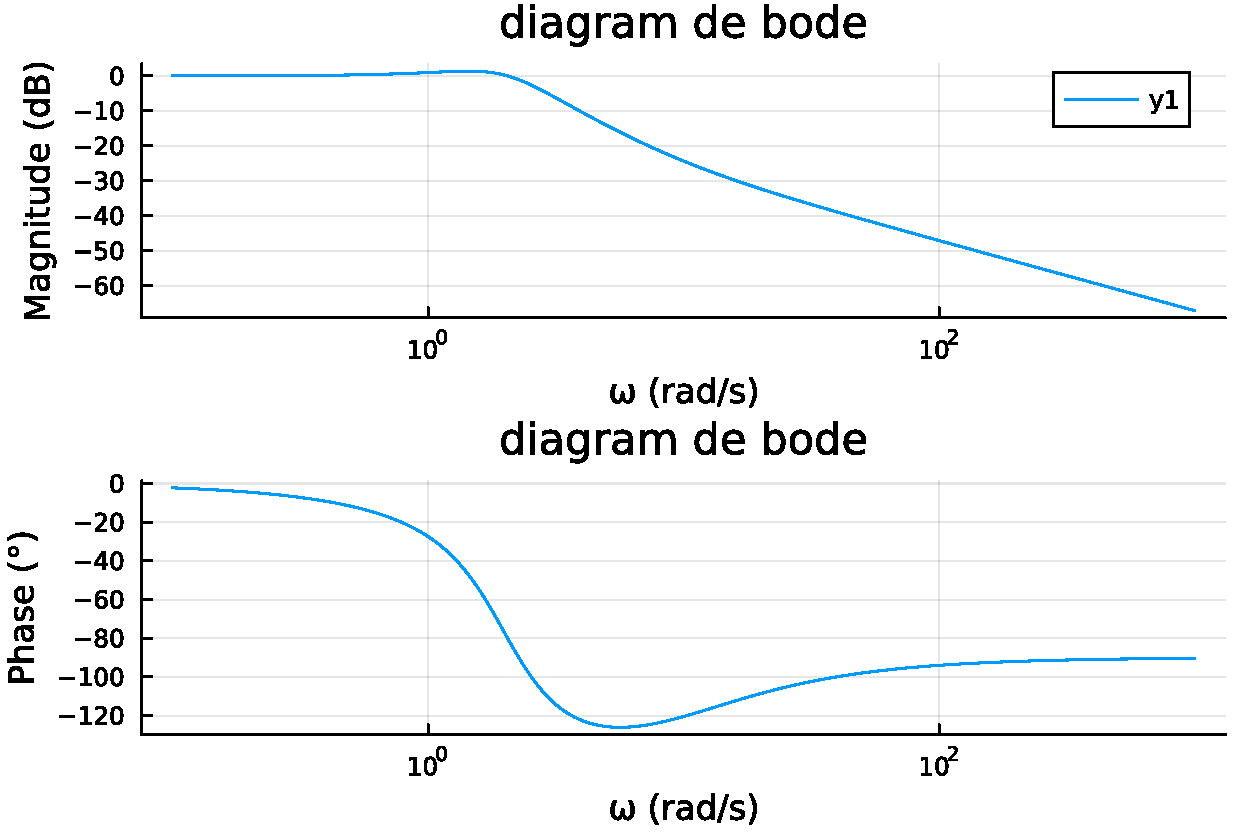
\includegraphics[width=0.95\textwidth]{../code/jlplots/Q3.pdf}
  \end{center}
  \caption{}\label{fig:bode}
\end{figure}

\end{document}
